\documentclass[10pt,a4paper]{article}
\usepackage[T1]{fontenc}
\usepackage{lmodern}
\usepackage{amssymb}
\usepackage[margin=2cm]{geometry}
\usepackage{graphicx}
\usepackage{booktabs}
\usepackage{float}
\usepackage{tabularx}
\usepackage{array}
\setlength{\parskip}{4pt}
\setlength{\parindent}{0pt}
\begin{document}
\begin{center}{\Large\bfseries Aircraft range optimiser: demo run 'impossible'}\\[4pt]
{\small Generated by scripts/demo\_report.py on 2026-11-26 20:22. Augmented Lagrangian + BFGS (our own code), checked with SciPy SLSQP.}\end{center}
\section{Your inputs}
\begin{table}[H]\centering\small
\begin{tabular}{lrr}
\toprule
\textbf{Input} & \textbf{Value} & \textbf{737-800 default} \\
\midrule
Passengers (100 kg each incl. bags) & 213 & 162 \\
Maximum take-off mass [kg] & 60,000 & 79,016 \\
Cruise altitude [ft] & 35,000 & 35,000 \\
Engine fuel burn factor & 1.0 & 1.0 \\
Maximum stall speed [m/s] & 64.0 & 64.0 \\
Maximum cruise Mach & 0.8 & 0.8 \\
Wing structure factor & 1.0 & 1.0 \\
Maximum wingspan [m] & no limit & no limit \\
Start: wingspan [m] & 34.32 & 34.32 \\
Start: wing area [m\textsuperscript{2}] & 124.6 & 124.6 \\
Start: cruise Mach & 0.785 & 0.785 \\
Start: cruise fuel [kg] & 17,000 & 17,000 \\
\bottomrule
\end{tabular}
\end{table}
\section{Designs}
\begin{table}[H]\centering\small
\begin{tabular}{lrr}
\toprule
\textbf{} & \textbf{Your start} & \textbf{Best attempt} \\
\midrule
Range [km] & 4,751 & 44 \\
Wingspan [m] & 34.3 & 21.6 \\
Wing area [m\textsuperscript{2}] & 124.6 & 94.0 \\
Aspect ratio & 9.45 & 4.98 \\
Cruise Mach & 0.785 & 0.800 \\
Cruise fuel [kg] & 17,000 & 185 \\
Initial mass [kg] & 82,371 & 62,658 \\
Wing mass [kg] & 5,849 & 2,952 \\
Tank capacity [kg] & 20,816 & 18,811 \\
L/D & 17.16 & 12.25 \\
Stall speed [m/s] & 63.8 & 64.1 \\
\bottomrule
\end{tabular}
\end{table}
The 737-800 cannot carry this payload within this MTOW, so it is not shown.

\textbf{Your starting design is NOT allowed.} It breaks: MTOW (by 37.3 \%). Its range is what it would fly, but it is not an acceptable aircraft.

\section{Result}
\textbf{No design satisfies all the requirements} (smallest violation reached 4.4e-02). The requirements contradict each other, e.g. too much payload for the MTOW, or a stall speed so low that no wing within the bounds meets it.

\begin{figure}[H]\centering
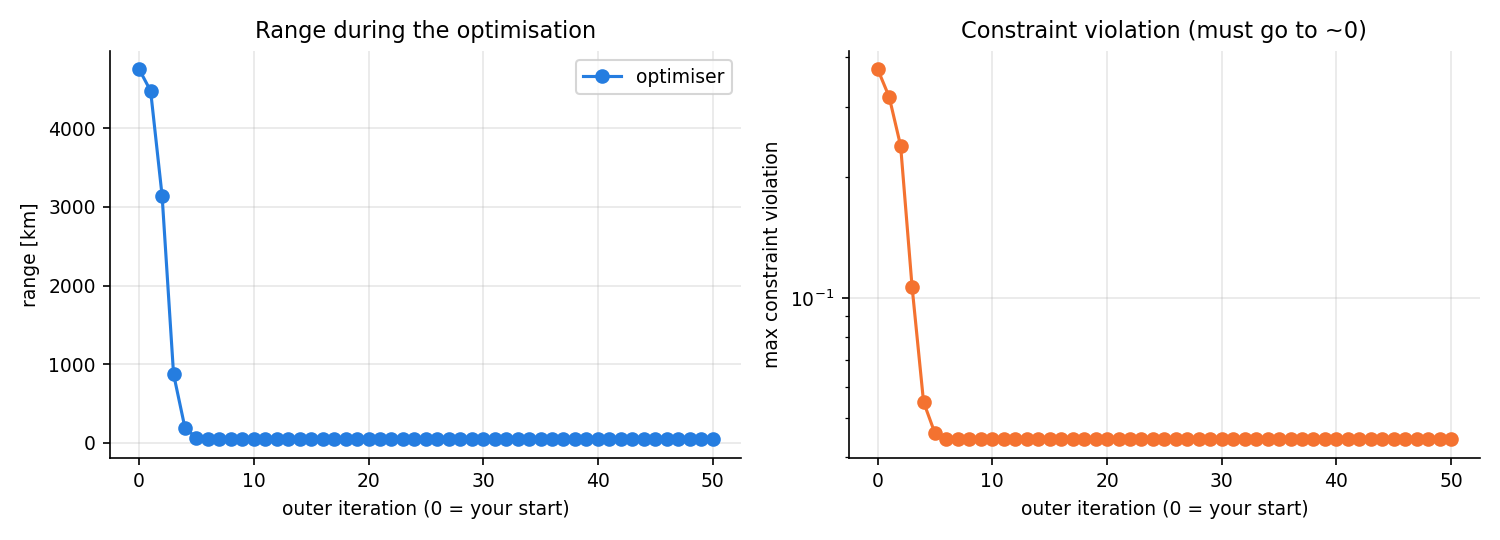
\includegraphics[width=0.9\textwidth]{fig_history.png}
\par\small\textit{Range and constraint violation at every outer iteration (0 = your start). An infeasible start can fly 'further' until the violation is forced to zero.}
\end{figure}
\section{Limits of this model}
Conceptual model calibrated on the 737-800: Breguet cruise, no wave drag (Mach cap instead), empirical wing mass and tank volume. Numbers are model predictions, not a validated aircraft.

\end{document}